\chapter{The \Lw{} Radiative Transfer Framework}\label{Chap:Lw}
% spell-checker: disable
%TC:group pycode 0 0
\begin{pycode}[Lw]
name = 'Lightweaver'
chLw = texfigure.Manager(
    pytex,
    './01aFlareModelling',
    number=4,
    python_dir='./01aFlareModelling/python',
    fig_dir=   './01aFlareModelling/Figs',
    data_dir=  './Data/01aFlareModelling'
)
\end{pycode}
% spell-checker: enable


The \Lw{} framework\footnote{\Lw{} is freely available under the permissive MIT license on GitHub (\url{https://github.com/Goobley/Lightweaver}) with archival on Zenodo.} \citep{Osborne2021, LightweaverZenodo} is a Python package built around a C++ core in which we have implemented the methods for numerical NLTE radiative transfer discussed in Sec.~\ref{Sec:IntroRT}.
As can be seen from the referencing of this section, none of these methods are novel on their own -- they represent the most robust methods encountered in our survey of NLTE radiative transfer -- and it is in the combination of these methods and the implementation strategies employed that \Lw{} differs from current \Sota{} radiative transfer codes.
An overview of the key components and functions that users will typically interact with is presented in \citet{Osborne2021}, in the following we describe the most important design decisions made in \Lw{} and explain how they can enable new forms of radiative transfer simulations whilst also increasing productivity.

\section{Philosophy}

The design of the \Lw{} framework is inspired by deep learning frameworks, such as PyTorch \citep{PyTorch}.
These have risen to prominence in recent years, due to their low barrier to entry, whilst still providing a customisable, full-featured, interface to the underlying methods that can be manipulated with pure Python code.
Machine learning frameworks provide a collection of building blocks that can be combined in multiple ways to allow researchers to construct new tools, specifically tailored to the problem they wish to address.
Whilst there can be slight performance gains from using a specialised, optimised, \Sota{} method implemented in a performance-focused language for this particular task, the benefits are likely outweighed by the additional development time.
This is especially true in research environments where tools are often used by a small group of researchers in a transient fashion, and the return on \emph{possible} optimisations is rarely sufficiently large compared to the benefits of increased development speed that a framework allows.
The use of a tested framework also allows researchers confidence in the core numerics they are reusing, whether they understand every detail or not.

The steps involved in solving the NLTE radiative transfer problem, e.g. formal solution, calculation of preconditioned rates, population updates, conservation of charge, and calculation of the PRD line profile ratio, are quite modular, and we provide optimised methods for the most commonly used steps following the standard techniques outlined previously.
They are building blocks that can be combined in different ways, to produce different tools.
These building blocks are the core offering of the \Lw{} framework, and are intended to be combined by the user in a new Python program to solve their particular problem.
If at any point a user wishes to fully replace a core component of \Lw{}, this can be done in Python, inside their program, with no modification the framework itself, whilst the other components can continue to be used as before.
This flexibility is encompassed by one of the core design goals, which is to allow Python code written by the user to ``interfere'' with all of the numerical treatment of the NLTE problem.

All other radiative transfer codes that the author has interacted with have been designed with a strict limit of one simulation per computer process.
Whilst this limitation does make the design of the program easier, especially in Fortran and C, it is not beneficial to an end user who may, for example, wish to couple multiple simulations with different atomic configurations, or, say, use one as a radiative boundary condition for another.
This latter configuration is applied extensively in Chap.~\ref{Chap:2DRT} where plane-parallel models are used as boundary conditions for a two-dimensional slab.
Whilst there are other solutions to this problem, such as saving necessary data and loading it in a reconfigured program, these are typically more error-prone than a simple program which can flexibly represent the coupling between these models in its code, even allowing for memory sharing of certain components.
To this end, each radiative transfer simulation performed in \Lw{} occurs in a self-contained \texttt{Context}, a Python object containing all necessary configuration and storage needed for this model.
These can be serialised using the \texttt{pickle} package of the Python standard library, allowing for a complete simulation to be dumped to disk or transferred between processes using the standard approach expected in the Python ecosystem.
This has impacts on parallelisation which will be discussed in Sec.~\ref{Sec:LwParallelisation}.

\section{Accessibility \& Code Overview}\label{Sec:LwCodeOverview}

One of the aims of \Lw{} is to attempt to reduce the barrier to entry for new users, thus we ensure that it is simple to install with pre-compiled libraries available.
Thus a user with a Python environment (version $\ge3.8$) using an x86-64 CPU supporting AVX vector extensions (essentially any Intel or AMD chip from the past decade) on any of macOS\footnote{Preliminary support of Apple's ARM CPUs is present, but several underlying libraries do not yet support this.}, Windows, or Linux, can install the package in one command using the Python package manager \texttt{pip}.
No additional compilation steps are necessary, and any additional libraries required are automatically sourced during installation.
Whilst slight performance benefits can likely be acquired by using a modern compiler to tune the code generated to the user's machine (and this option is available for advanced users), the option of automatically installing a tested release version of the library in under \SI{60}{\second} was an important goal that has easily been achieved thanks to Python's well-supported packaging systems.

All interfaces to the framework are thoroughly documented through the Python docstring convention (internally to the source files) and can be used to automatically generate HTML or \LaTeX{} documentation.
This can also be viewed online at \url{https://goobley.github.io/Lightweaver}.

As of v0.7.3, excluding automatically generated code (of which we make extensive use), the \Lw{} frontend consists of 4520 lines of Python, with 2326 lines of comments and documentation.
777 of these consist of an implementation of the equation of state originally authored by Wittmann following \citet{Mihalas1978}, and ported to Python by J. de la Cruz Rodriguez (used here with permission).
This is an LTE equation of state that has been used in both the SIR \citep{1992RuizCobo} and NICOLE \citep{Socas-Navarro2015} codes.

The backend consists of 9896 code lines of personally authored C++, along with two external libraries: Faddeeva\footnote{\url{http://ab-initio.mit.edu/wiki/index.php/Faddeeva_Package}} (Steven G. Johnson, 2066 lines of code, MIT license) used for computing Voigt functions, and a lightweight multi-platform thread pool and scheduler\footnote{\url{https://github.com/vurtun/lib/blob/master/sched.h}} (Doug Binks \& Micha Mettke, 788 lines of code, zlib license).
As both of these libraries are small and permissively licensed, they are included directly in \Lw{}'s distribution, so there is no concern about these links going stale.
Multiple routines present in the calculation of the background terms are thread-safe reimplementations of those used in RH \citep{Uitenbroek2001}, with permission.
There are also 2439 lines of Cython \citep{Behnel2011} code present in the backend.
Cython is a compiled language used to bridge the Python interfaces to the C++ core.
It allows us to share NumPy \citep{Harris2020} arrays by reference between Python and C++, allowing changes to the array's contents to be visible from either language with no duplication necessary.
This data sharing is not just efficient but allows the Python frontend to be ``involved'' with the radiative transfer calculations on a deep level in line with \Lw{}'s design goals.

\section{Model Atoms}

An oft-quoted aphorism in programming circles is that of \emph{Greenspun's tenth rule of programming}\footnote{e.g. \url{https://philip.greenspun.com/research/}} which states: ``Any sufficiently complicated C or Fortran program contains an ad hoc, informally-specified, bug-ridden, slow implementation of half of Common Lisp''.
The implementations of model atoms in the codes the author is personally familiar with are examples of this.
This is not to say that configuration files containing the data needed to run a program are problematic, but we are instead referring to the large amount of logic associated with these files, that eventually turns into an \emph{ad hoc} domain specific language.
These models are structured and contain methods of specifying the approximations to be used for different terms, such as van der Waals broadening and bound-free cross sections.
Any new method that a user wishes to implement then has to be added to the custom interpreter responsible for parsing these files and propagating this information into the numeric core of the program.

A different approach to the problem of needing to specify data with \emph{associated} methods and approximations is to define a set of requirements (henceforth \emph{contract}) specifying the information needed by the numerical core and allow the specific model to fulfil this contract through any means.
It is this approach we take in \Lw{}.
This means that model atoms need to be ``smart'' and have the ability to execute arbitrary code.
Implementing these models in Python makes this trivial, and its wide array of scientific libraries are also available\footnote{We stress that other languages could be used for this task, and they need not be dynamic ``scripting'' languages; for example, a similar approach could be achieved in C/C++ through the use of dynamic libraries.}.
As a ``free bonus'', thanks to the models being standard Python objects stored in source code, the Python interpreter will take care of parsing these models, through extremely well-tested code paths.

An \texttt{AtomicModel} in \Lw{} is the definition of an object containing an element or isotope identifier, and a list of each of levels, lines, continua, and collisional rate approximations.
Each of these terms is itself a Python object which must conform to a particular contract describing the form of the information it must be capable of supplying when a particular method is called.
Many of these objects also contain components with their own contracts.
These contracts are defined through the use of Python classes, and a basic implementation of features, comparable to those in extant radiative transfer codes, is present within the core of  \Lw{}.
These can be further extended with new functionality through the use of inheritance.
A user can therefore implement a new method for computing, say, the absorption profile \citep[e.g. the non-Voigt profile of][]{Kowalski2017} of a spectral line and employ this by defining a new model atom with no changes needed in the \Lw{} package.

Atomic models can be supplied in two different ways, in textual source code, which is both human and machine readable, or in a \texttt{pickle}, which is only machine readable, possibly from a previously serialised \texttt{Context}.
The former of these is treated as a canonical form, and it can always be recovered by asking Python for the representation of the object (via the \texttt{repr} function).
This imposes a minor constraint on the way user constructed classes extending the components of these models need to be defined i.e. they must define a \texttt{\_\_repr\_\_} function defining how to recover a textual representation of themselves.
This is due to our adherence to the standard Python convention that \texttt{obj == eval(repr(obj))}, requiring that the evaluation (in the Python interpreter) of the textual representation of an object give an equivalent object.
This is explained in depth with the examples provided in \citet{Osborne2021}.

The use of Python objects and data structures to describe the model atoms does not only allow the models to execute arbitrary code, but also for the models to be manipulated via user code.
This makes managing and modifying atomic models easier as transformations (modifications of parameters) can be undertaken in bulk by code, rather than a painstaking manual process.
This is all achieved through the use of standard Python, with no custom code needed to support this.

\section{Other Implementation Details}

Here we present a general overview of the implementation of some of the techniques discussed in Sec.~\ref{Sec:IntroRT}, primarily from a design and usage perspective, rather than a numerical one, as we find the former to be more insightful.
The numerical implementation details of \Lw{}, including ensuring correct normalisation of the numerical integrations performed are presented in depth in \citet{Osborne2021}.
In general we follow the best practices discussed in literature, and given the amount of memory present in today's computers we typically opt for slightly more memory costly approaches if they are significantly simpler or more efficient.
In the plane-parallel case, a Gauss-Legendre quadrature based on the polar angle of the rays is typically used for integrating terms with angular dependence, although a user can supply their own that is optimised to a particular problem.
Integrations over frequency are typically carried out by using a simple Riemann sum variant, such as the midpoint rule, and ensuring normalisation of terms such as the line absorption profile and PRD scattering integral.

In \Lw{}, model atoms are considered \emph{active}, \emph{detailed static}, or \emph{passive}.
Prior to construction of the \texttt{Context}, the user defines the set of model atoms, and how each is to be treated in this particular simulation.
This is done through an instance of the \texttt{RadiativeSet} class.
Active atoms are given the full NLTE treatment, with the terms necessary for iterating the populations (the preconditioned $\Gamma$ matrix) being computed with the formal solution.
To correctly resolve the effects of Doppler shifts, the emissivity and opacity terms associated with the transitions of these atoms are considered to be angle-dependent, and are computed for each ray in the angular quadrature, both up- and downgoing.
So-called detailed static atoms are treated similarly, but the terms for updating the populations are not computed.
As such, they will be ignored by the population update routines.
A model atom defined as detailed static is intended to be used when the atomic populations of a species are known \emph{a priori}, e.g., it is in LTE, or its populations determined in an alternative manner but its transitions are a significant source of emissivity and opacity that may affect another species being simulated (and the radiative terms associated with this other species is not expected to have a significant effect on the former).
Model atoms designated as passive are treated in LTE and only their bound-free transitions are considered.
Their contributions to the plasma emissivity and opacity are considered isotropic and incorporated into the background terms.
The populations of all of these species are stored in a \texttt{SpeciesStateTable}, which holds the arrays that are shared with the C++ iteration machinery.

To handle overlapping transitions, we treat all of these on a common grid.
This grid is computed by the instance of \texttt{RadiativeSet}, after the treatment of each atom has been defined.
The wavelength grids of each transition considered in detail are combined, and the region of this common grid associated with each transition is used in the evaluation of its line absorption profile or photoionisation cross-section.
During the formal solution, all of the sources of emissivity and opacity present at each wavelength (active, detailed static, and passive model atoms, along with other background terms) are summed to provide the total emissivity and opacity terms needed to compute the source function.

As discussed in Sec.~\ref{Sec:LwCodeOverview}, the background emissivity, opacity, and scattering terms take the same form as those in RH.
The background implementation is defined through a flexible interface that receives the atomic populations, model atoms, and wavelength at which the background parameters need to be known.
Through this interface, a user can easily override the implementation provided with RH.
In all of the numerical experiments presented in this thesis the default implementation (or its parallel cousin \texttt{FastBackground}) is used.
The components considered in the default background implementation and their original references are:
\begin{itemize}
    \itemsep-0.5em
    \item Frequency independent Thomson scattering \citep{Mihalas1978}
    \item H free-free \citep{Mihalas1978}
    \item H$_2^-$ free-free \citep{Bell1980}
    \item H$_2^+$ free-free \citep{Bates1952}
    \item H$_2$ Rayleigh scattering \citep{Victor1969,Tarafdar1973}
    \item H$^-$ bound-free \citep{Geltman1962,Mihalas1978}
    \item H$^-$ free-free \citep{Stilley1970,Mihalas1978}
    \item H$^-$ free-free ($>\SI{9113}{\nano\m}$) \citep{John1988}
    \item basic Rayleigh scattering for H and He \citep{Mihalas1978}
    \item OH bound-free \citep{Kurucz1987}
    \item CH bound-free \citep{Kurucz1987}
    \item Bound-free terms from all passive atoms.
\end{itemize}
We note that the terms with \citep{Mihalas1978} as their reference are also discussed similarly in \citep{Hubeny2014}.
Due to its importance in obtaining a correct background opacity, the molecular H$^-$ population is always computed.
\Lw{} can compute the formation of molecules, assuming that they form in instantaneous chemical equilibrium.
Their formation will reduce the total populations of the species bound up in them, and may contribute to the background opacities (e.g. CH, OH, H$_2$).

In \Lw{}, the time-dependent population updates are computing using the fully implicit variant of the method described in Sec.~\ref{Sec:TimeDepPopUpdates}, i.e. with $\theta=1$.
In general, we have found no difference between the fully- and semi-implicit treatments of the term, and adopt $\theta=1$ for simplicity.
It is simple to replace the time-dependent population update scheme with one that performs the semi-implicit integration without modifying the core of \Lw{} itself.

The derivatives of the collisional rates needed for the Newton-Raphson charge conservation scheme are computed by a finite-difference approximation.
This is relatively efficient as these rates depend only on local parameters, and much less restrictive than requiring a user to also compute the analytic derivative of any collisional rate formalisms they add to their own model atoms.

As discussed in Sec.~\ref{Sec:ShortChar}, we adopt a short-characteristics formal solver to solve the RTE, and in \Lw{}, the default implementation for plane-parallel atmospheres is the cubic Bézier spline technique of \citet{DelaCruzRodriguez2013}.
We also provide an implementation of the simple linear short-characteristics scheme, and allow for users to load their own formal solvers from shared libraries at runtime, provided they implement the interface described by the \Lw{} codebase.

\section{Parallelisation}\label{Sec:LwParallelisation}

The self-contained nature of the \texttt{Context} makes \Lw{} programs for computing grids of models easy to adapt to paradigms such as the Message Passing Interface \citep[MPI, e.g.][for an overview of the MPICH implementation]{Gropp1996} commonly used in high performance computing environments.
A proof of concept implementation utilising MPI for a grid of models was undertaken by A. Asensio Ramos (\emph{private communication}), running 10,000 models in 4 hours across 15 CPUs with no need to modify \Lw{}.

A secondary form of parallelisation is also incorporated into \Lw{}.
This consists of splitting time-consuming work from a single simulation over multiple threads in the same machine.
This work primarily consists of the formal solution, accumulation of terms into the $\Gamma$ matrix, and calculation of any line profile ratios needed for PRD, which are parallelised over wavelength
These terms typically represent the vast majority of the program's runtime for non-trivial simulations.
The calculation of line absorption profiles, when using atomic models with the default Voigt profile implementation, along with the optional \texttt{FastBackground} implementation of background opacities, emissivities, and scatterings, are also parallelised.
The choices of the terms to parallelise has been motivated by our observations of the most time-consuming processes when using \Lw{} to undertake the numerical experiments presented in Chaps.~\ref{Chap:TimeDepRt} and \ref{Chap:2DRT}.


\section{Validation}\label{Sec:LwValidation}

The \Lw{} framework was extensively validated during development, primarily against RH \citep{Uitenbroek2001}, but also the synthesis module of SNAPI \citep{Milic2018} when discrepancies were found.
RH is a well-established code that serves as a cornerstone of NLTE radiative transfer in the solar physics community.
It assumes a single time-independent atmospheric input, for which the statistical equilibrium solution of the atomic populations is computed.
The MALI method with full preconditioning \citep{Rybicki1992} is used, and implementations of angle-averaged and angle-dependent PRD and cross-redistribution are present following the methods outlined in \citet{Uitenbroek2001,MillerRicci2002}.
RH can also be used for NLTE modelling of molecular lines, but we do not make use of this here.
In the examples presented here, we make use of v2 of the RH code, distributed by H. Uitenbroek, and not the massively parallel RH 1.5D presented in \citet{Pereira2015}.

The synthesis module of SNAPI also uses a MALI method allowing for overlapping lines, with an implementation of the method entirely distinct to the one used in RH.
It assumes a CRD treatment of all spectral lines.
In the following we will present just a few of the validation cases that have been used during the development of \Lw{}.

%spell-checker: disable
\setpythontexautoprint{false}
\begin{pycode}[Lw]
import lightweaver as lw
from lightweaver.rh_atoms import H_6_atom, C_atom, O_atom,  Si_atom, Al_atom, CaII_atom, Fe_atom, He_atom, MgII_atom, Mg_atom, N_atom, Na_atom, S_atom
from helita.sim.rh import Rhout
from lightweaver.fal import Falc82
import astropy.units as u

atmos = Falc82()
atmos.quadrature(5)

aSet = lw.RadiativeSet([H_6_atom(), C_atom(), O_atom(), Si_atom(), Al_atom(),
                        CaII_atom(), Fe_atom(), He_atom(), Mg_atom(), N_atom(),
                        Na_atom(), S_atom()])
aSet.set_active('H', 'Ca')
spect = aSet.compute_wavelength_grid()

molPaths = [lw.get_default_molecule_path() + m + '.molecule' for m in ['H2']]
mols = lw.MolecularTable(molPaths)

eqPops = aSet.compute_eq_pops(atmos, mols)
ctx = lw.Context(atmos, spect, eqPops, Nthreads=8)
for i in range(5):
    ctx.formal_sol_gamma_matrices()

for i in range(300):
    dJ = ctx.formal_sol_gamma_matrices()
    dPops = ctx.stat_equil()

    if dJ < 3e-3 and dPops < 1e-3:
        break

atmos = Falc82()
atmos.quadrature(5)
eqPopsChargeCons = aSet.iterate_lte_ne_eq_pops(atmos, mols)
ctxCc = lw.Context(atmos, spect, eqPopsChargeCons, Nthreads=8, conserveCharge=True)
for i in range(5):
    ctxCc.formal_sol_gamma_matrices()

for i in range(300):
    dJ = ctxCc.formal_sol_gamma_matrices()
    dPops = ctxCc.stat_equil()

    if dJ < 3e-3 and dPops < 1e-3:
        break

atmos = Falc82()
atmos.quadrature(5)
eqPopsLte = aSet.iterate_lte_ne_eq_pops(atmos, mols)
ctxLte = lw.Context(atmos, spect, eqPopsLte, Nthreads=8, conserveCharge=False)
for i in range(5):
    ctxLte.formal_sol_gamma_matrices()

for i in range(300):
    dJ = ctxLte.formal_sol_gamma_matrices()
    dPops = ctxLte.stat_equil()

    if dJ < 3e-3 and dPops < 1e-3:
        break

wave = np.linspace(853.9444, 854.9444, 1001)
Iwave = ctx.compute_rays(wave, 1.0)
IwaveCc = ctxCc.compute_rays(wave, 1.0)
IwaveLte = ctxLte.compute_rays(wave, 1.0)

rh = Rhout(chLw.data_file('LwRhComparison/RhConfigAndOutput'))
rh.read_ray(chLw.data_file('LwRhComparison/RhConfigAndOutput/spectrum_1.00'))

ca = CaII_atom()
lambda0 = ca.lines[4].lambda0
fig = plt.figure(figsize=texfigure.figsize(pytex, scale=1.0, height_ratio=0.55))
plt.plot(rh.wave - lambda0, rh.int, label='RH')
plt.plot(wave - lambda0, Iwave, '--', label='Lightweaver')
plt.plot(wave - lambda0, IwaveLte, label='Lightweaver LTE $n_e$')
plt.plot(wave - lambda0, IwaveCc, label='Lightweaver Charge Cons.')
plt.xlabel(r'$\Delta\lambda$ [nm]')
plt.ylabel(r'Intensity [J\,m$^{-2}$\,s$^{-1}$\,Hz$^{-1}$\,sr$^{-1}$]')
plt.xlim(wave[0] - lambda0, wave[-1] - lambda0)
plt.legend(frameon=False)
lFig = chLw.save_figure('LwRhComparison', fig, fext='.pgf')
lFig.caption = r'Comparison of \Lw{} and RH synthesis of \CaLine{} from the FALC atmosphere with different electron density solutions.'
lFig.placement = 'htbp'
\end{pycode}
\begin{pycode}[Lw]

_, atmos = lw.read_multi_atmos(chLw.data_file('FalSillyVelRunRh/FalVelocityLte.atmos'))
atmos.quadrature(5)

aSet = lw.RadiativeSet([H_6_atom(), C_atom(), O_atom(), Si_atom(), Al_atom(),
                        CaII_atom(), Fe_atom(), He_atom(), Mg_atom(), N_atom(),
                        Na_atom(), S_atom()])
aSet.set_active('Ca')
spect = aSet.compute_wavelength_grid()

molPaths = [lw.get_default_molecule_path() + m + '.molecule' for m in ['H2']]
mols = lw.MolecularTable(molPaths)

eqPops = aSet.compute_eq_pops(atmos, mols)
ctx = lw.Context(atmos, spect, eqPops, Nthreads=8)
for i in range(5):
    ctx.formal_sol_gamma_matrices()

for i in range(300):
    dJ = ctx.formal_sol_gamma_matrices()
    dPops = ctx.stat_equil()

    if dJ < 3e-3 and dPops < 1e-3:
        break

wave = np.linspace(853.9444, 854.9444, 1001)
Iwave = ctx.compute_rays(wave, 1.0)

rh = Rhout(chLw.data_file('FalSillyVelRunRh'))
rh.read_ray(chLw.data_file('FalSillyVelRunRh/spectrum_1.00'))

snapi = np.loadtxt(chLw.data_file('snapi_test_8542.dat'))
snapiWl = lw.air_to_vac(snapi[:, 0] * 1e7)
snapiI = lw.convert_specific_intensity(snapiWl,
                                       snapi[:, 1] << u.erg*u.cm**(-3)*u.s**(-1)*u.sr**(-1),
                                       'J/m2/s/Hz/sr')
# NOTE(cmo): SNAPI uses cgs for _everything_, wavelength, specific intensity... _everything_.

ca = CaII_atom()
lambda0 = ca.lines[4].lambda0
fig = plt.figure(figsize=texfigure.figsize(pytex, scale=1.0, height_ratio=0.55))
plt.plot(rh.wave - lambda0, rh.int, label='RH')
plt.plot(wave - lambda0, Iwave, '--', label='Lightweaver')
plt.plot(snapiWl - lambda0, snapiI, '-.', label='SNAPI')
plt.xlabel(r'$\Delta\lambda$ [nm]')
plt.ylabel(r'Intensity [J\,m$^{-2}$\,s$^{-1}$\,Hz$^{-1}$\,sr$^{-1}$]')
# plt.xlim(wave[0] - lambda0, wave[-1] - lambda0)
plt.xlim(-0.45, 0.45) # slightly smaller grid to stay within SNAPI range.
plt.legend(frameon=False)
lFig = chLw.save_figure('LwValidationSillyVel', fig, fext='.pgf')
lFig.caption = r'Comparison of the \Lw{}, RH, and SNAPI synthesis of \CaLine{} from the FALC atmosphere with complex velocity profile and LTE electron density.'
lFig.placement = 'htbp'
\end{pycode}
\begin{pycode}[Lw]

_, atmos = lw.read_multi_atmos(chLw.data_file('RadynSnapT05NoPrd/Flat1e9NoIncRad_t05.atmos'))
atmos.quadrature(5)

aSet = lw.RadiativeSet([H_6_atom(), C_atom(), O_atom(), Si_atom(), Al_atom(),
                        CaII_atom(), Fe_atom(), He_atom(), MgII_atom(), N_atom(),
                        Na_atom(), S_atom()])
aSet.set_active('H', 'Ca')
spect = aSet.compute_wavelength_grid()

molPaths = [lw.get_default_molecule_path() + m + '.molecule' for m in ['H2']]
mols = lw.MolecularTable(molPaths)

eqPops = aSet.compute_eq_pops(atmos, mols)
ctx = lw.Context(atmos, spect, eqPops, Nthreads=16)
for i in range(5):
    ctx.formal_sol_gamma_matrices()

for i in range(300):
    dJ = ctx.formal_sol_gamma_matrices()
    dPops = ctx.stat_equil()

    if dJ < 3e-3 and dPops < 1e-3:
        break

eqPopsPrd = aSet.compute_eq_pops(atmos, mols)
ctxPrd = lw.Context(atmos, spect, eqPopsPrd, Nthreads=16, hprd=False)
for i in range(5):
    ctxPrd.formal_sol_gamma_matrices()

for i in range(300):
    dJ = ctxPrd.formal_sol_gamma_matrices()
    dPops = ctxPrd.stat_equil()
    dRho = ctxPrd.prd_redistribute()

    if dJ < 3e-3 and dPops < 1e-3:
        break

# eqPopsHPrd = aSet.compute_eq_pops(atmos, mols)
# ctxHPrd = lw.Context(atmos, spect, eqPopsHPrd, Nthreads=16, hprd=True)
# for i in range(5):
#     ctxHPrd.formal_sol_gamma_matrices()

# for i in range(300):
#     dJ = ctxHPrd.formal_sol_gamma_matrices()
#     dPops = ctxHPrd.stat_equil()
#     dRho = ctxHPrd.prd_redistribute()

#     if dJ < 3e-3 and dPops < 1e-3:
#         break

wave = np.linspace(393.377, 393.577, 1001)
Iwave = ctx.compute_rays(wave, 1.0)
IwavePrd = ctxPrd.compute_rays(wave, 1.0)
# IwaveHPrd = ctxHPrd.compute_rays(wave, 1.0)

rh = Rhout(chLw.data_file('RadynSnapT05NoPrd'))
rh.read_ray(chLw.data_file('RadynSnapT05NoPrd/spectrum_1.00'))
rhPrd = Rhout(chLw.data_file('RadynSnapT05Prd'))
rhPrd.read_ray(chLw.data_file('RadynSnapT05Prd/spectrum_1.00'))

ca = CaII_atom()
lambda0 = ca.lines[1].lambda0
fig = plt.figure(figsize=texfigure.figsize(pytex, scale=1.0, height_ratio=0.55))
plt.plot(rh.wave - lambda0, rh.int, label='RH CRD')
plt.plot(wave - lambda0, Iwave, '--', label='Lightweaver CRD')
plt.plot(rhPrd.wave - lambda0, rhPrd.int, label='RH PRD')
plt.plot(wave - lambda0, IwavePrd, '--', label='Lightweaver PRD')
# plt.plot(wave - lambda0, IwaveHPrd, '--', label='Lightweaver PRD (Angle Approximate)')
plt.yscale('log')
plt.xlabel(r'$\Delta\lambda$ [nm]')
plt.ylabel(r'Intensity [J\,m$^{-2}$\,s$^{-1}$\,Hz$^{-1}$\,sr$^{-1}$]')
plt.ylim(1e-10, None)
# plt.xlim(wave[0] - lambda0, wave[-1] - lambda0)
plt.xlim(-0.09, 0.09)
plt.legend(frameon=False)
lFig = chLw.save_figure('LwValidationPrd', fig, fext='.pgf')
lFig.caption = r'Comparison of \Lw{} and RH synthesis of \Caii{} K from a RADYN snapshot comparing the effects of PRD.'
lFig.placement = 'htb'
\end{pycode}
\begin{pycode}[Lw]
from lightweaver.rh_atoms import H_4_atom
from matplotlib.ticker import MaxNLocator
from lightweaver.atomic_model import reconfigure_atom
from copy import deepcopy

Prd = False

# NOTE(cmo): Use the H4 atom with constant collisional ionisation/excitation
# strengths from 7000K, as done by Phil Judge. Replace temperature (i.e.
# Maxwellian) varying Johnson (1972) rates with just this one rate.
h4 = H_4_atom()
newCols = []
for c in h4.collisions:
    col = deepcopy(c)
    col.temperature = [c.temperature[2], c.temperature[3]]
    col.rates = [c.rates[2], c.rates[2]]
    newCols.append(col)
h4.collisions = newCols
reconfigure_atom(h4)

def iterate_ctx(ctx, prd=True, Nscatter=3, NmaxIter=500):
    for i in range(NmaxIter):
        dJ = ctx.formal_sol_gamma_matrices()
        if i < Nscatter:
            continue
        delta = ctx.stat_equil()
        if prd:
            dRho = ctx.prd_redistribute(maxIter=5)

        if dJ < 3e-3 and delta < 1e-3:
            print(i)
            print('----------')
            return

atmos = Falc82()
atmos.quadrature(5)
if Prd:
    aSet = lw.RadiativeSet([H_6_atom(), C_atom(), O_atom(), Si_atom(), Al_atom(), CaII_atom(), Fe_atom(), He_atom(), MgII_atom(), N_atom(), Na_atom(), S_atom()])
else:
    aSet = lw.RadiativeSet([h4, C_atom(), O_atom(), Si_atom(), Al_atom(), CaII_atom(), Fe_atom(), He_atom(), MgII_atom(), N_atom(), Na_atom(), S_atom()])
aSet.set_active('H')
spect = aSet.compute_wavelength_grid()

eqPops = aSet.compute_eq_pops(atmos)
# eqPops = aSet.iterate_lte_ne_eq_pops(atmos)
ctx = lw.Context(atmos, spect, eqPops,
                 hprd=Prd, conserveCharge=False, Nthreads=8)
iterate_ctx(ctx, prd=Prd)

print('Achieved initial Stat Eq')

dt = 0.1
NtStep = int(60 / dt)
NsubStep = 100

prevT = np.copy(atmos.temperature)
for i in range(11, 31):
    di = (i - 20.0) / 3.0
    atmos.temperature[i] *= 1.0 + 2.0 * np.exp(-di**2)

hPops = [np.copy(eqPops['H'])]
subIters = []
for it in range(NtStep):
    ctx.update_deps()

    prevState = None
    for sub in range(NsubStep):
        dJ = ctx.formal_sol_gamma_matrices()
        delta, prevState = ctx.time_dep_update(dt, prevState, ngUpdate=None)
        # deltaNr = ctx.nr_post_update(timeDependentData={'dt': dt, 'nPrev': prevState})
        # delta = max(delta, deltaNr)
        if Prd:
            ctx.prd_redistribute(maxIter=5)

        if delta < 1e-3 and dJ < 3e-3:
            subIters.append(sub)
            break
    else:
        raise ValueError('No converge')

    hPops.append(np.copy(eqPops['H']))
    print('Iteration %d (%f s) done after %d sub iterations' % (it, (it+1)*dt, sub))


initialAtmos = Falc82()

fig, ax = plt.subplots(2,2, sharex=True, figsize=texfigure.figsize(pytex, scale=0.93, height_ratio=0.6))
ax = ax.flatten()
cmass = np.log10(atmos.cmass/1e1)

lowerIdx = np.searchsorted(cmass, -4.936)
upperIdx = np.searchsorted(cmass, -4.930)

ax[0].plot(cmass[lowerIdx:upperIdx], initialAtmos.temperature[lowerIdx:upperIdx], 'r', label='Initial', lw=0.8)
ax[0].plot(cmass[lowerIdx:upperIdx], atmos.temperature[lowerIdx:upperIdx], '-+b', label='Final', lw=0.8, markeredgewidth=0.6, markersize=4)
ax[0].legend(frameon=False)

for p in hPops[1::10]:
    ax[1].plot(cmass[lowerIdx:upperIdx], np.log10(p[0, lowerIdx:upperIdx]/1e6), 'k', lw=0.5)
    ax[2].plot(cmass[lowerIdx:upperIdx], np.log10(p[1, lowerIdx:upperIdx]/1e6), 'k', lw=0.5)
    ax[3].plot(cmass[lowerIdx:upperIdx], np.log10(p[-1, lowerIdx:upperIdx]/1e6), 'k', lw=0.5)

p = hPops[0]
ax[1].plot(cmass[lowerIdx:upperIdx], np.log10(p[0, lowerIdx:upperIdx]/1e6), 'r', lw=0.8)
ax[2].plot(cmass[lowerIdx:upperIdx], np.log10(p[1, lowerIdx:upperIdx]/1e6), 'r', lw=0.8)
ax[3].plot(cmass[lowerIdx:upperIdx], np.log10(p[-1, lowerIdx:upperIdx]/1e6), 'r', lw=0.8)

p = hPops[-1]
ax[1].plot(cmass[lowerIdx:upperIdx], np.log10(p[0, lowerIdx:upperIdx]/1e6),  '-+b', lw=0.8, markersize=4, markeredgewidth=0.6)
ax[2].plot(cmass[lowerIdx:upperIdx], np.log10(p[1, lowerIdx:upperIdx]/1e6),  '-+b', lw=0.8, markersize=4, markeredgewidth=0.6)
ax[3].plot(cmass[lowerIdx:upperIdx], np.log10(p[-1,lowerIdx:upperIdx]/1e6), '-+b', lw=0.8, markersize=4, markeredgewidth=0.6)

ax[0].set_xlim(-4.935, -4.931)
ax[0].xaxis.set_major_locator(MaxNLocator(3))
ax[0].set_ylim(0, 6e4)
ax[1].set_ylim(6, 11)
ax[2].set_ylim(1, 6.25)
ax[3].set_ylim(10, 11)

ax[2].set_xlabel('$\log\,m$ [cm$^{-2}$]')
ax[3].set_xlabel('$\log\,m$ [cm$^{-2}$]')

ax[0].set_ylabel('$T$ [K]')
ax[1].set_ylabel('$\log\,n(n=1)$ [cm$^{-3}$]')
ax[2].set_ylabel('$\log\,n(n=2)$ [cm$^{-3}$]')
ax[3].set_ylabel('$\log\,n(\kappa)$ [cm$^{-3}$]')

# fig.tight_layout()
fig.subplots_adjust(hspace=0.13, wspace=0.38, bottom=0.12)

lFig = chLw.save_figure('LwValidationJudge', fig, fext='.pgf')
lFig.caption = r'Validation of the time-dependent population update scheme in \Lw{}. Compare with Fig.~\ref{Fig:Judge2017Original}. Each black line shows the population densities once every \SI{1}{\second}.'
lFig.short_caption = r"Validation of \Lw{}'s time-dependent population update scheme."
lFig.placement = 'p'
\end{pycode}
\setpythontexautoprint{true}

\begin{pycode}[Lw]
from ReadAtmost import read_atmost
import zarr

atmost = read_atmost(chLw.data_file('Flat1e9NoIncRad/atmost.dat'))
atmost.to_SI()

data = zarr.convenience.open(chLw.data_file('Flat1e9NoIncRad/Flat1e9NoIncRadLIThesis.zip'), 'r')

timesToPlot = [5, 11, 20, 40]
fig, ax = plt.subplots(2, 2, figsize=texfigure.figsize(pytex, scale=1.0, height_ratio=0.7))
ax = ax.ravel()

for i, a in enumerate(ax):
    time = timesToPlot[i]
    radynIdx = np.searchsorted(atmost.time, time)
    lwIdx = np.searchsorted(data['time'][...], time)

    label = 'RADYN' if i == 0 else None
    a.semilogy(atmost.z1[radynIdx] / 1e6, atmost.ne1[radynIdx], label=label)
    label = 'Lightweaver' if i == 0 else None
    a.semilogy(atmost.z1[radynIdx] / 1e6, data['ne'][lwIdx], '--', label=label)
    a.set_xlim(None, 2.8)
    a.set_title('{:.2f} s'.format(time))

    if i in [0, 2]:
        a.set_ylabel(r'$n_e$ [m$^{-3}$]')
    else:
        a.set_yticklabels([])

    if i in [2, 3]:
        a.set_xlabel(r'$z$ [Mm]')
    else:
        a.set_xticklabels([])

ax[0].legend(frameon=False)
fig.tight_layout()

lFig = chLw.save_figure('LwValidationTimeDepNe', fig, fext='.pgf')
lFig.caption = r'Comparison of electron density in a RADYN simulation and time-dependent reprocessing using \Lw{} that will be presented as the F9 model of Chap.~\ref{Chap:TimeDepRt}.'
lFig.short_caption = r'Validation of time-dependent charge conservation in \Lw{}.'
lFig.placement = 'ht'
\end{pycode}

\py[Lw]|chLw.get_figure('LwRhComparison')|
\py[Lw]|chLw.get_figure('LwValidationSillyVel')|

%spell-checker: enable

Fig.~\ref{Fig:LwRhComparison} presents a comparison of the synthesis of \CaLine{} by \Lw{} and RH in the FALC atmosphere of \citet{Fontenla1993}.
This is a static, semi-empirical quiet Sun atmosphere, so the synthesis is performed in statistical equilibrium.
RH's solution is shown in blue, with the \Lw{} solution overlaid in dashed orange.
There is clearly very good agreement between these codes in this simple static test.
This figure also shows the sensitivity of \CaLine{} to the electron density when computed under the assumption of LTE ionisation (green), and how the the charge conservation method implemented in \Lw{} can help to mitigate these effects when the electron density is not known \emph{a priori} (red).
The line profile computed from the simulation with the charge conservation strategy approaches the reference solution, where the electron density is provided by the FAL model.
The primary differences between these treatments is likely due to other species, such as Fe, being treated in LTE.

In Fig.~\ref{Fig:LwValidationSillyVel} we once again present the synthesis of \CaLine{} in the FALC atmosphere, but here a complex velocity profile is imposed on the atmospheric model.
The vertical velocity structure of the atmosphere is defined to be two periods of a sine wave with amplitude \SI{30}{\kilo\metre\per\second} mapped over the vertical extent of the FALC model (approximately \SI{2}{\mega\metre}).
The electron density is set and held fixed at the value given by the LTE ionisation state of the plasma.
This is to allow for easier comparison between the codes with different formulations for their model atmospheres.
Here RH's solution is once again shown in blue, \Lw{}'s in dashed orange, and SNAPI's in dot-dashed green.
This problem serves primarily as a test of the formal solver: the piecewise parabolic method of \citet{Auer1994} implemented in RH, which falls back to monotonic linear interpolation if the parabolic terms under- or overshoot, was unable to correctly solve the problem, causing the iteration to fail.
The cubic Bézier method of \citet{DelaCruzRodriguez2013} normally used in all three of these codes, along with their standard MALI iteration machinery, provides a very similar solution in all three cases.
The slight differences apparent around $\Delta\lambda=\SI{-0.1}{\nano\metre}$ is likely to be caused by differences in the formal solver implementations; the version implemented in RH uses the method of \citet{Fritsch1984} to compute numerical estimates of the necessary derivatives, whereas we use the method of \citet{Steffen1990} in \Lw{} following the recommendation of \citet{Janett2018}, as the accuracy of \citet{Fritsch1984} falls to first-order on non-uniform grids.
Additionally, the implementation present in RH chooses to limit the control points on the spline interpolants to positive values, but following the advice of de la Cruz Rodríguez (\emph{private communication}) we remove this limitation as negative absorption can occur with sufficient stimulated emission.
The differences between SNAPI and the other methods around $\Delta\lambda=\SI{0.02}{\nano\metre}$ is also likely due to choices made when estimating the derivatives and limiting the control points.
SNAPI also uses a different formulation for the background emissivities and opacities, as well as parametrisations for the damping terms present in the Voigt profile.
These are likely responsible for the differences in the $|\Delta\lambda| \geq \SI{0.15}{\nano\metre}$ far wing to continuum region.
Nevertheless, we consider that the agreement between the three implementations is very good on this challenging test.

\py[Lw]|chLw.get_figure('LwValidationPrd')|

Fig.~\ref{Fig:LwValidationPrd} shows a simple validation test for the PRD method implemented in \Lw{}.
We show the synthesis of the \Caii{} K line in statistical equilibrium from a snapshot of a \Radyn{} simulation.
This snapshot is taken from the F9 simulation discussed in Chap.~\ref{Chap:TimeDepRt}, at \SI{5}{\second} after flare heating starts.
The CRD solutions are shown in blue and dashed orange for RH and \Lw{} respectively.
The PRD solutions both employ angle-averaged PRD and are presented in green (RH) and dashed red (\Lw{}).
The agreement between these solutions is again very good, with a slight observable difference around $|\Delta\lambda=\SI{0.012}{\nano\metre}|$ where the line in \Lw{}'s PRD solution appears slightly wider than in RH's.
This difference is present only over a very small range of wavelengths and we consider the agreement between the two implementations to be very good.

\begin{figure}[p]
    \centering
    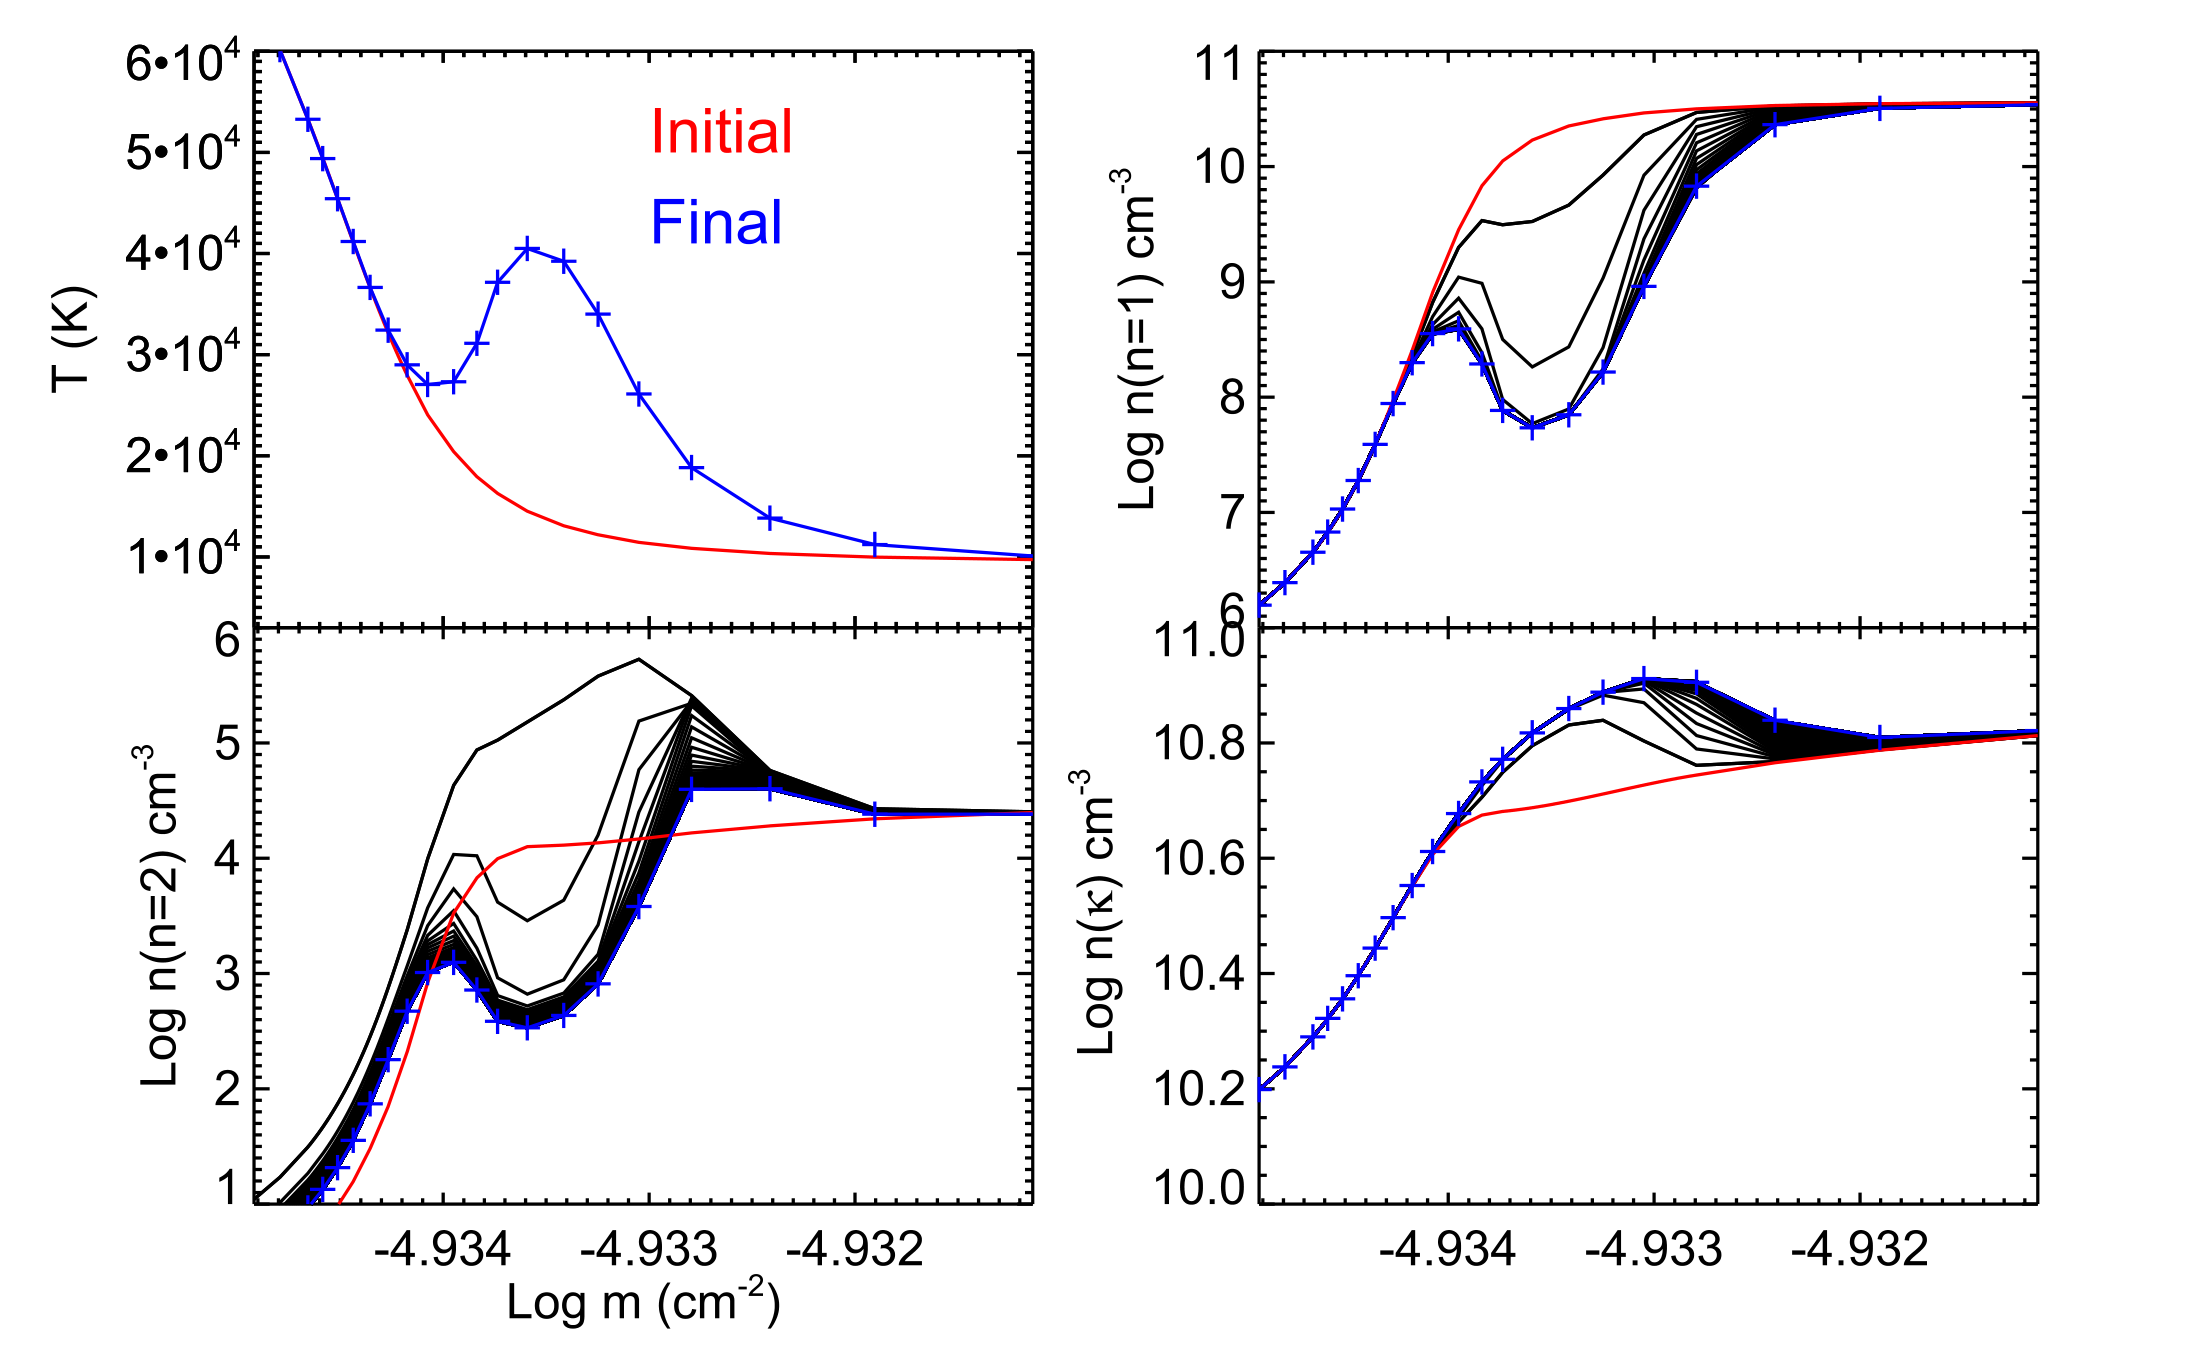
\includegraphics[width=0.85\columnwidth]{01aFlareModelling/StaticFigs/Judge2017Fig4.png}
    \caption[Fig. 4 of Judge (2017). Time-dependent response of hydrogen populations to instantaneous temperature change.]{Fig. 4 of \citet{Judge2017}. The response of hydrogen levels ($n=1, 2$) and continuum ($\kappa$) are shown for an instantaneous perturbation of the temperature of the FALC model (top-left panel). Each black line shows the population densities once every \SI{1}{\second}. © AAS. Reproduced with permission.}
    \label{Fig:Judge2017Original}
\end{figure}
\py[Lw]|chLw.get_figure('LwValidationJudge')|

Slightly more complex examples are needed to test the time-dependent machinery present in \Lw{}, and neither SNAPI nor RH, with their time-independent viewpoints can be used for comparison here.
We instead use the example of a perturbed FALC atmosphere presented by \citet{Judge2017}.
This figure is reproduced here as Fig.~\ref{Fig:Judge2017Original}.
After converging to the statistical equilibrium solution in a standard FALC atmosphere, the temperature is perturbed as shown by the blue line of the top-left panel of both Fig.~\ref{Fig:Judge2017Original} and our own solution presented in Fig.~\ref{Fig:LwValidationJudge}.
This model uses a three level plus continuum model hydrogen atom, and the populations of the ground, first excited, and continuum states are shown in the top-right, bottom-left, and bottom-right panels of these figures respectively.
The red line shows their starting values, and the blue line their final values after the simulation has been allowed to run for \SI{500}{\second} in the case of Fig.~\ref{Fig:Judge2017Original} and \SI{60}{\second} for Fig.~\ref{Fig:LwValidationJudge}, as we find the solution has stabilised by this point.
The black lines represent the solutions for each population every \SI{1}{\second}.
The $x$-axis on these plots is the atmospheric column mass, and Fig.~\ref{Fig:LwValidationJudge} is prepared in cgs to allow direct comparison to Fig.~\ref{Fig:Judge2017Original}.
The typically temperature-dependent (i.e. due to assuming a Maxwellian electron distribution) collisional ionisation and excitation ``strengths'' are fixed to their values at \SI{7000}{\kelvin} obtained using the method of \citet{Johnson1972} (P. Judge, \emph{private communication}; we note that the collisional \emph{rates} associated with these still scale with $\sqrt{T}$).

We see good overall agreement with \citet{Judge2017}, but the differences are larger than those presented in the previous figures.
The method used by \citet{Judge2017} is different to ours, and uses full preconditioning but with a $\Lambda$ operator based on the escape probability formalism of \citet{Hummer1982}, using a one-sided escape probability.
This approach is much more approximate than the full MALI treatment applied in \Lw{}, as it only performs the approximate formal solution at one wavelength per transition, and computes the integrals over wavelength and angle analytically.
The advantage of this treatment is that it is much less computationally intensive.
Thus, the use of this approximate method by \citet{Judge2017} is likely to be the origin of the differences between our results, and we find that the level populations converge to similar final solutions, at apparently similar rates.
The most substantial difference between our results is for the $n=2$ population: in Fig.~\ref{Fig:Judge2017Original}, the points close to a column mass of \SI{-4.9315}{\per\square\centi\metre} do not vary from their initial values, whereas in our model they change quite dramatically, with an enhancement of up to 2\,dex, leaving the range of the original plot, but converge close to the expected final solution.
This is likely an effect of downgoing radiation not being considered in the escape probability based formal solution of \citet{Judge2017}.
The maximum enhancement in this level also peaks higher than that seen in Fig.~\ref{Fig:Judge2017Original}, but rapidly drops towards the expected solution.
The downgoing radiation is also likely responsible for the offset of the final populations from the initial model in the \SI{-4.9315}{\per\square\centi\m} region that is not present, as the populations stay stable when the populations are advanced in time through the same process without the temperature perturbation, i.e. statistical equilibrium is maintained.
This simple example illustrates that \Lw{}'s behaviour is reasonable when applied to time-dependent problems, and the quality of its treatment will become apparent in the in-depth comparisons with \Radyn{} presented in Chap.~\ref{Chap:TimeDepRt}.

\py[Lw]|chLw.get_figure('LwValidationTimeDepNe')|

In Fig.~\ref{Fig:LwValidationTimeDepNe} we show the electron density in the lower atmosphere at four different timesteps of a \Radyn{} simulation where the radiative transfer (including self-consistent electron density) has been reprocessed using \Lw{}.
The techniques used here will be described in depth in Chap.~\ref{Chap:TimeDepRt}, and this figure is produced using the F9 model described in Sec.~\ref{Sec:CaiiRadynSims}.
The \Lw{} model presented is run with time-dependent charge conservation, maintaining self-consistency throughout the remainder of the simulation, whilst loading the other thermodynamic parameters from the \Radyn{} model at each timestep, and using these to compute the time-dependent population updates and self-consistent electron density.
Advection of the atomic populations and electron density is performed using a similar technique to \Radyn{}, implemented as per Sec.~\ref{Sec:MsLwAdvection}.
The electron density in the \Radyn{} model is shown in blue, and the \Lw{} model in dashed orange.
The agreement between the two models is extremely good, including the fine features around $z=\SI{1.2}{\mega\metre}$ shown in the \SI{11}{\second} panel.

\Lw{} agrees well with the other models against which it has been tested here; it is easy to construct new validation tests for statistical equilibrium cases that can be run with many different extant radiative transfer codes, but the validation of time-dependent treatments on their own is more difficult, due to current tools often coupling these equations to hydrodynamics.
Other tests have been undertaken to verify the performance of \Lw{}, but those presented here should be sufficient to demonstrate its capabilities.


\section{\emph{Lightspinner}}

During the development of \Lw{}, a simpler pedagogic framework was also constructed.
This framework, \emph{Lightspinner}\footnote{Available on GitHub (\url{https://github.com/Goobley/Lightspinner}), with archival on Zenodo.} \citep{Lightspinner}, is written in pure Python and focuses on documenting the internal numerics of a simple formal solver and the MALI method using full preconditioning (under the assumption of CRD).
It is accompanied by a slide deck highlighting the most important terms that need to be understood to implement these methods following \citet{Rybicki1992} and \citet{Uitenbroek2001} for iteration, and \citet{Olson1987} and \citet{Auer1994} for the short-characteristics formal solver (although only a linear formal solver is implemented in the code). This framework can be employed to help users familiarise themselves with the concepts of NLTE radiative transfer and some of the techniques present in \Lw{}; it presents the core concepts clearly, and naïvely, without focusing on performance, so can easily be dismantled and understood by a single person over the course of a few days.

\section{Discussions}

We have presented a description and validation of the \Lw{} radiative transfer framework and the intentions behind its design.
Frameworks can substantially enhance productivity, and enable the construction of specialised tools without the need to focus on the implementation or performance of the common core of dense numerical code shared by programs of this style.
The power of this will be demonstrated with the experiments presented in Chapters~\ref{Chap:TimeDepRt} and \ref{Chap:2DRT} which leverage \Lw{} significantly, and demonstrate how the addition of small amounts of Python can yield tools that would otherwise require in-depth modification and coupling of existing tools such as RH and \Radyn{}.